\documentclass[14pt]{extbook}
\usepackage{multicol, enumerate, enumitem, hyperref, color, soul, setspace, parskip, fancyhdr} %General Packages
\usepackage{amssymb, amsthm, amsmath, latexsym, units, mathtools} %Math Packages
\everymath{\displaystyle} %All math in Display Style
% Packages with additional options
\usepackage[headsep=0.5cm,headheight=12pt, left=1 in,right= 1 in,top= 1 in,bottom= 1 in]{geometry}
\usepackage[usenames,dvipsnames]{xcolor}
\usepackage{dashrule}  % Package to use the command below to create lines between items
\newcommand{\litem}[1]{\item#1\hspace*{-1cm}\rule{\textwidth}{0.4pt}}
\pagestyle{fancy}
\lhead{Progress Quiz 6}
\chead{}
\rhead{Version C}
\lfoot{9689-6866}
\cfoot{}
\rfoot{Spring 2021}
\begin{document}

\begin{enumerate}
\litem{
Write the equation of the line in the graph below in Standard form $Ax+By=C$. Then, choose the intervals that contain $A, B, \text{ and } C$.
\begin{center}
    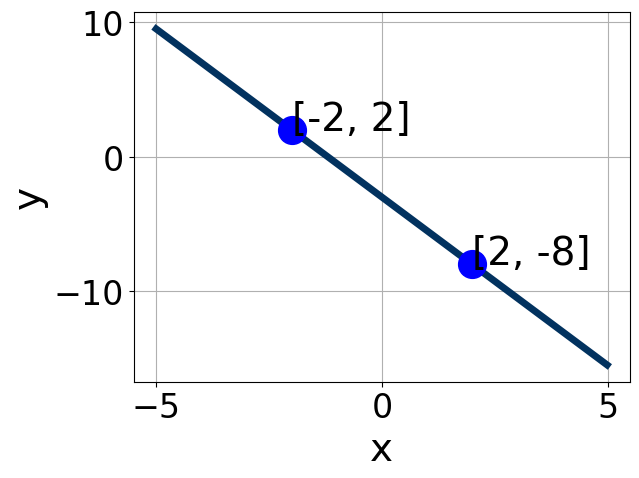
\includegraphics[width=0.5\textwidth]{../Figures/linearGraphToStandardC.png}
\end{center}
\begin{enumerate}[label=\Alph*.]
\item \( A \in [-4.5, 1.5], \hspace{3mm} B \in [-1.75, -0.66], \text{ and } \hspace{3mm} C \in [2.8, 5.3] \)
\item \( A \in [-6, -4], \hspace{3mm} B \in [1.93, 2.18], \text{ and } \hspace{3mm} C \in [-7.2, -4.5] \)
\item \( A \in [2, 7], \hspace{3mm} B \in [1.93, 2.18], \text{ and } \hspace{3mm} C \in [-7.2, -4.5] \)
\item \( A \in [-4.5, 1.5], \hspace{3mm} B \in [0.94, 1.4], \text{ and } \hspace{3mm} C \in [-5.8, -0.6] \)
\item \( A \in [2, 7], \hspace{3mm} B \in [-2.8, -1.51], \text{ and } \hspace{3mm} C \in [5.5, 9] \)

\end{enumerate} }
\litem{
Find the equation of the line described below. Write the linear equation as $ y=mx+b $ and choose the intervals that contain $m$ and $b$.\[ \text{Parallel to } 8 x + 3 y = 7 \text{ and passing through the point } (-5, 2). \]\begin{enumerate}[label=\Alph*.]
\item \( m \in [-2.67, -0.67] \hspace*{3mm} b \in [5, 8] \)
\item \( m \in [1.67, 7.67] \hspace*{3mm} b \in [12.33, 16.33] \)
\item \( m \in [-2.67, -0.67] \hspace*{3mm} b \in [-16.33, -7.33] \)
\item \( m \in [-1.38, 2.62] \hspace*{3mm} b \in [-16.33, -7.33] \)
\item \( m \in [-2.67, -0.67] \hspace*{3mm} b \in [11.33, 13.33] \)

\end{enumerate} }
\litem{
First, find the equation of the line containing the two points below. Then, write the equation as $ y=mx+b $ and choose the intervals that contain $m$ and $b$.\[ (-10, 11) \text{ and } (-11, -9) \]\begin{enumerate}[label=\Alph*.]
\item \( m \in [18, 25] \hspace*{3mm} b \in [210, 215] \)
\item \( m \in [-25, -17] \hspace*{3mm} b \in [-231, -225] \)
\item \( m \in [18, 25] \hspace*{3mm} b \in [19, 24] \)
\item \( m \in [18, 25] \hspace*{3mm} b \in [-212, -206] \)
\item \( m \in [18, 25] \hspace*{3mm} b \in [0, 5] \)

\end{enumerate} }
\litem{
Write the equation of the line in the graph below in Standard form $Ax+By=C$. Then, choose the intervals that contain $A, B, \text{ and } C$.
\begin{center}
    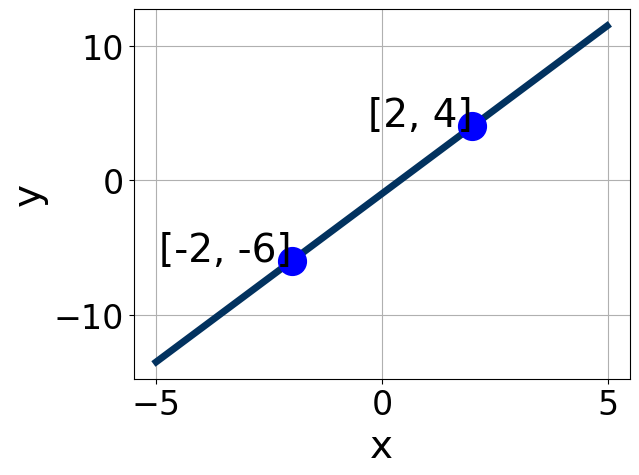
\includegraphics[width=0.5\textwidth]{../Figures/linearGraphToStandardCopyC.png}
\end{center}
\begin{enumerate}[label=\Alph*.]
\item \( A \in [1.4, 4.4], \hspace{3mm} B \in [-5.2, -4.84], \text{ and } \hspace{3mm} C \in [-30, -17] \)
\item \( A \in [-0.7, 1.7], \hspace{3mm} B \in [-2.64, -0.41], \text{ and } \hspace{3mm} C \in [-7, -1] \)
\item \( A \in [1.4, 4.4], \hspace{3mm} B \in [4.05, 7.36], \text{ and } \hspace{3mm} C \in [22, 31] \)
\item \( A \in [-0.7, 1.7], \hspace{3mm} B \in [0.1, 1.48], \text{ and } \hspace{3mm} C \in [3, 7] \)
\item \( A \in [-3.4, -1.8], \hspace{3mm} B \in [-5.2, -4.84], \text{ and } \hspace{3mm} C \in [-30, -17] \)

\end{enumerate} }
\litem{
Solve the equation below. Then, choose the interval that contains the solution.\[ -6(2x -8) = -19(18x -5) \]\begin{enumerate}[label=\Alph*.]
\item \( x \in [0.35, 0.41] \)
\item \( x \in [0.42, 0.51] \)
\item \( x \in [0.1, 0.18] \)
\item \( x \in [-0.48, -0.38] \)
\item \( \text{There are no real solutions.} \)

\end{enumerate} }
\litem{
Solve the linear equation below. Then, choose the interval that contains the solution.\[ \frac{-3x -6}{8} - \frac{-5x + 9}{4} = \frac{-4x + 4}{5} \]\begin{enumerate}[label=\Alph*.]
\item \( x \in [-1.45, 0.24] \)
\item \( x \in [10.88, 11.83] \)
\item \( x \in [1.85, 2.59] \)
\item \( x \in [-0.28, 0.81] \)
\item \( \text{There are no real solutions.} \)

\end{enumerate} }
\litem{
First, find the equation of the line containing the two points below. Then, write the equation as $ y=mx+b $ and choose the intervals that contain $m$ and $b$.\[ (2, 3) \text{ and } (-2, 2) \]\begin{enumerate}[label=\Alph*.]
\item \( m \in [-0.2, 2.8] \hspace*{3mm} b \in [-2.64, -2.4] \)
\item \( m \in [-0.2, 2.8] \hspace*{3mm} b \in [3.62, 4.4] \)
\item \( m \in [-2.5, 0.1] \hspace*{3mm} b \in [1.08, 2.11] \)
\item \( m \in [-0.2, 2.8] \hspace*{3mm} b \in [1.62, 3.41] \)
\item \( m \in [-0.2, 2.8] \hspace*{3mm} b \in [0.57, 1.23] \)

\end{enumerate} }
\litem{
Find the equation of the line described below. Write the linear equation as $ y=mx+b $ and choose the intervals that contain $m$ and $b$.\[ \text{Parallel to } 9 x + 5 y = 3 \text{ and passing through the point } (5, -8). \]\begin{enumerate}[label=\Alph*.]
\item \( m \in [1.21, 2.36] \hspace*{3mm} b \in [-17.7, -15.6] \)
\item \( m \in [-2.25, -1.14] \hspace*{3mm} b \in [-1.6, -0.1] \)
\item \( m \in [-1.26, 0.15] \hspace*{3mm} b \in [0.4, 1.5] \)
\item \( m \in [-2.25, -1.14] \hspace*{3mm} b \in [0.4, 1.5] \)
\item \( m \in [-2.25, -1.14] \hspace*{3mm} b \in [-13.5, -12] \)

\end{enumerate} }
\litem{
Solve the linear equation below. Then, choose the interval that contains the solution.\[ \frac{7x + 4}{7} - \frac{-3x + 7}{4} = \frac{9x + 5}{6} \]\begin{enumerate}[label=\Alph*.]
\item \( x \in [-6.95, -4.95] \)
\item \( x \in [5.05, 12.05] \)
\item \( x \in [31, 34] \)
\item \( x \in [1.01, 6.01] \)
\item \( \text{There are no real solutions.} \)

\end{enumerate} }
\litem{
Solve the equation below. Then, choose the interval that contains the solution.\[ -2(8x -4) = -16(14x + 15) \]\begin{enumerate}[label=\Alph*.]
\item \( x \in [-0.98, -0.85] \)
\item \( x \in [-1.21, -1.16] \)
\item \( x \in [-1.18, -1.06] \)
\item \( x \in [1.1, 1.21] \)
\item \( \text{There are no real solutions.} \)

\end{enumerate} }
\end{enumerate}

\end{document}